%%%%%%%%%%%%%%%%%%%%%%%%%%%%%%%%%%%
%This is the LaTeX ARTICLE template for RSC journals
%Copyright The Royal Society of Chemistry 2016
%%%%%%%%%%%%%%%%%%%%%%%%%%%%%%%%%%%

\documentclass[twoside,twocolumn,9pt]{article}
\usepackage{extsizes}
\usepackage[super,sort&compress,comma]{natbib} 
\usepackage[version=3]{mhchem}
\usepackage[left=1.5cm, right=1.5cm, top=1.785cm, bottom=2.0cm]{geometry}
\usepackage{balance}
\usepackage{mathptmx}
\usepackage{sectsty}
\usepackage{graphicx} 
\usepackage{lastpage}
\usepackage[format=plain,justification=justified,singlelinecheck=false,font={stretch=1.125,small,sf},labelfont=bf,labelsep=space]{caption}
\usepackage{float}
\usepackage{fancyhdr}
\usepackage{fnpos}
\usepackage[english]{babel}
\addto{\captionsenglish}{%
  \renewcommand{\refname}{Notes and references}
}
\usepackage{array}
\usepackage{droidsans}
\usepackage{charter}
\usepackage[T1]{fontenc}
\usepackage[usenames,dvipsnames]{xcolor}
\usepackage{setspace}
\usepackage[compact]{titlesec}
\usepackage{hyperref}
%%%Please don't disable any packages in the preamble, as this may cause the template to display incorrectly.%%%


\usepackage{balance}
\usepackage{times,mathptmx}
\usepackage{sectsty}
\usepackage{graphicx} 
\usepackage{lastpage}
\usepackage[format=plain,justification=justified,singlelinecheck=false,font={stretch=1.125,small,sf},labelfont=bf,labelsep=space]{caption}
\usepackage{float}
\usepackage{fancyhdr}
\usepackage{fnpos}
\usepackage[english]{babel}
\addto{\captionsenglish}{%
  \renewcommand{\refname}{Notes and references}
}
\usepackage{array}
\usepackage{droidsans}
\usepackage{charter}
\usepackage[T1]{fontenc}
\usepackage[usenames,dvipsnames]{xcolor}
\usepackage{setspace}
\usepackage[compact]{titlesec}
\usepackage{hyperref}

\usepackage{abstract}
\usepackage{graphicx}
\usepackage{gensymb}
\usepackage{caption}
\usepackage{amsmath}
\usepackage{amsthm}
\usepackage{amsfonts}
%\usepackage{float}
\usepackage{sidecap}
\usepackage{mathtools}
\usepackage{adjustbox}
\usepackage{ upgreek }




\usepackage{epstopdf}%This line makes .eps figures into .pdf - please comment out if not required.

\definecolor{cream}{RGB}{222,217,201}

\begin{document}

\pagestyle{fancy}
\thispagestyle{plain}
\fancypagestyle{plain}{
%%%HEADER%%%
\renewcommand{\headrulewidth}{0pt}
}
%%%END OF HEADER%%%

%%%PAGE SETUP - Please do not change any commands within this section%%%
\makeFNbottom
\makeatletter
\renewcommand\LARGE{\@setfontsize\LARGE{15pt}{17}}
\renewcommand\Large{\@setfontsize\Large{12pt}{14}}
\renewcommand\large{\@setfontsize\large{10pt}{12}}
\renewcommand\footnotesize{\@setfontsize\footnotesize{7pt}{10}}
\makeatother

\renewcommand{\thefootnote}{\fnsymbol{footnote}}
\renewcommand\footnoterule{\vspace*{1pt}% 
\color{cream}\hrule width 3.5in height 0.4pt \color{black}\vspace*{5pt}} 
\setcounter{secnumdepth}{5}

\makeatletter 
\renewcommand\@biblabel[1]{#1}            
\renewcommand\@makefntext[1]% 
{\noindent\makebox[0pt][r]{\@thefnmark\,}#1}
\makeatother 
\renewcommand{\figurename}{\small{Fig.}~}
\sectionfont{\sffamily\Large}
\subsectionfont{\normalsize}
\subsubsectionfont{\bf}
\setstretch{1.125} %In particular, please do not alter this line.
\setlength{\skip\footins}{0.8cm}
\setlength{\footnotesep}{0.25cm}
\setlength{\jot}{10pt}
\titlespacing*{\section}{0pt}{4pt}{4pt}
\titlespacing*{\subsection}{0pt}{15pt}{1pt}
%%%END OF PAGE SETUP%%%

%%%FOOTER%%%
\fancyfoot{}
\fancyfoot[LO,RE]{\vspace{-7.1pt}\includegraphics[height=9pt]{head_foot/LF}}
\fancyfoot[CO]{\vspace{-7.1pt}\hspace{13.2cm}\includegraphics{head_foot/RF}}
\fancyfoot[CE]{\vspace{-7.2pt}\hspace{-14.2cm}\includegraphics{head_foot/RF}}
\fancyfoot[RO]{\footnotesize{\sffamily{1--\pageref{LastPage} ~\textbar  \hspace{2pt}\thepage}}}
\fancyfoot[LE]{\footnotesize{\sffamily{\thepage~\textbar\hspace{3.45cm} 1--\pageref{LastPage}}}}
\fancyhead{}
\renewcommand{\headrulewidth}{0pt} 
\renewcommand{\footrulewidth}{0pt}
\setlength{\arrayrulewidth}{1pt}
\setlength{\columnsep}{6.5mm}
\setlength\bibsep{1pt}
%%%END OF FOOTER%%%

%%%FIGURE SETUP - please do not change any commands within this section%%%
\makeatletter 
\newlength{\figrulesep} 
\setlength{\figrulesep}{0.5\textfloatsep} 

\newcommand{\topfigrule}{\vspace*{-1pt}% 
\noindent{\color{cream}\rule[-\figrulesep]{\columnwidth}{1.5pt}} }

\newcommand{\botfigrule}{\vspace*{-2pt}% 
\noindent{\color{cream}\rule[\figrulesep]{\columnwidth}{1.5pt}} }

\newcommand{\dblfigrule}{\vspace*{-1pt}% 
\noindent{\color{cream}\rule[-\figrulesep]{\textwidth}{1.5pt}} }

\makeatother
%%%END OF FIGURE SETUP%%%

%%%TITLE, AUTHORS AND ABSTRACT%%%
\twocolumn[
  \begin{@twocolumnfalse}
{\includegraphics[height=30pt]{head_foot/journal_name}\hfill\raisebox{0pt}[0pt][0pt]{\includegraphics[height=55pt]{head_foot/RSC_LOGO_CMYK}}\\[1ex]
\includegraphics[width=18.5cm]{head_foot/header_bar}}\par
\vspace{1em}
\sffamily
\begin{tabular}{m{4.5cm} p{13.5cm} }

\includegraphics{head_foot/DOI} & \noindent\LARGE{\textbf{A High-Throughput Computational Dataset of Halide Perovskite Alloys$^\dag$}} \\%Article title goes here instead of the text "This is the title"
\vspace{0.3cm} & \vspace{0.3cm} \\

 & \noindent\large{Jiaqi Yang,\textit{$^{a}$} Panayotis Manganaris\textit{$^{a}$} and Arun Mannodi-Kanakkithodi\textit{$^{a}$}} \\%Author names go here instead of "Full name", etc.

\includegraphics{head_foot/dates} & \noindent\normalsize{Novel halide perovskites with improved stability and optoelectronic properties can be designed via composition engineering at cation and/or anion sites. Data-driven methods, especially high-throughput first principles computations and subsequent analysis based on unique materials descriptors, are key to achieving this goal. In this work, we report a density functional theory (DFT)-based dataset of 550 ABX$_3$ halide perovskite compounds, with various atomic and molecular species considered at A, B and X sites, and different amounts of mixing considered at each site to simulate special quasirandom structures of alloys. We perform GGA-PBE calculations on pseudo-cubic perovskite structures to determine their lattice constants, stability in terms of formation and decomposition energies, electronic band gaps, and properties extracted from optical absorption spectra. To elucidate the importance of the level of theory used, we further perform 300 calculations using the more expensive HSE06 functional and determine lattice constant, stability and band gap, and compare PBE and HSE06 properties with some experimentally measured results. Trends in the datasets are unraveled in terms of the effects of mixing at different sites, the composition in terms of specific atomic or molecular species, and averaged elemental properties of species at different sites. This work presents the most comprehensive DFT perovskite alloy dataset to date and the data, which is open-source, can be exploited to train predictive and optimization models for accelerating the design of completely new compositions that may yield large solar cell efficiencies and improved performance across many optoelectronic applications.} 

\end{tabular}

 \end{@twocolumnfalse} \vspace{0.6cm}

  ]
%%%END OF TITLE, AUTHORS AND ABSTRACT%%%

%%%FONT SETUP - please do not change any commands within this section
\renewcommand*\rmdefault{bch}\normalfont\upshape
\rmfamily
\section*{}
\vspace{-1cm}


%%%FOOTNOTES%%%

\footnotetext{\textit{$^{a}$~School of Materials Engineering, Purdue University, West Lafayette, IN 47907, USA; E-mail: amannodi@purdue.edu }}

\footnotetext{\dag~Electronic Supplementary Information (ESI) available: [details of any supplementary information available should be included here]. See DOI: 00.0000/00000000.}


%%%END OF FOOTNOTES%%%

%%%MAIN TEXT%%%%


\section*{Introduction}

... \\


\begin{figure*}[h]
\centering
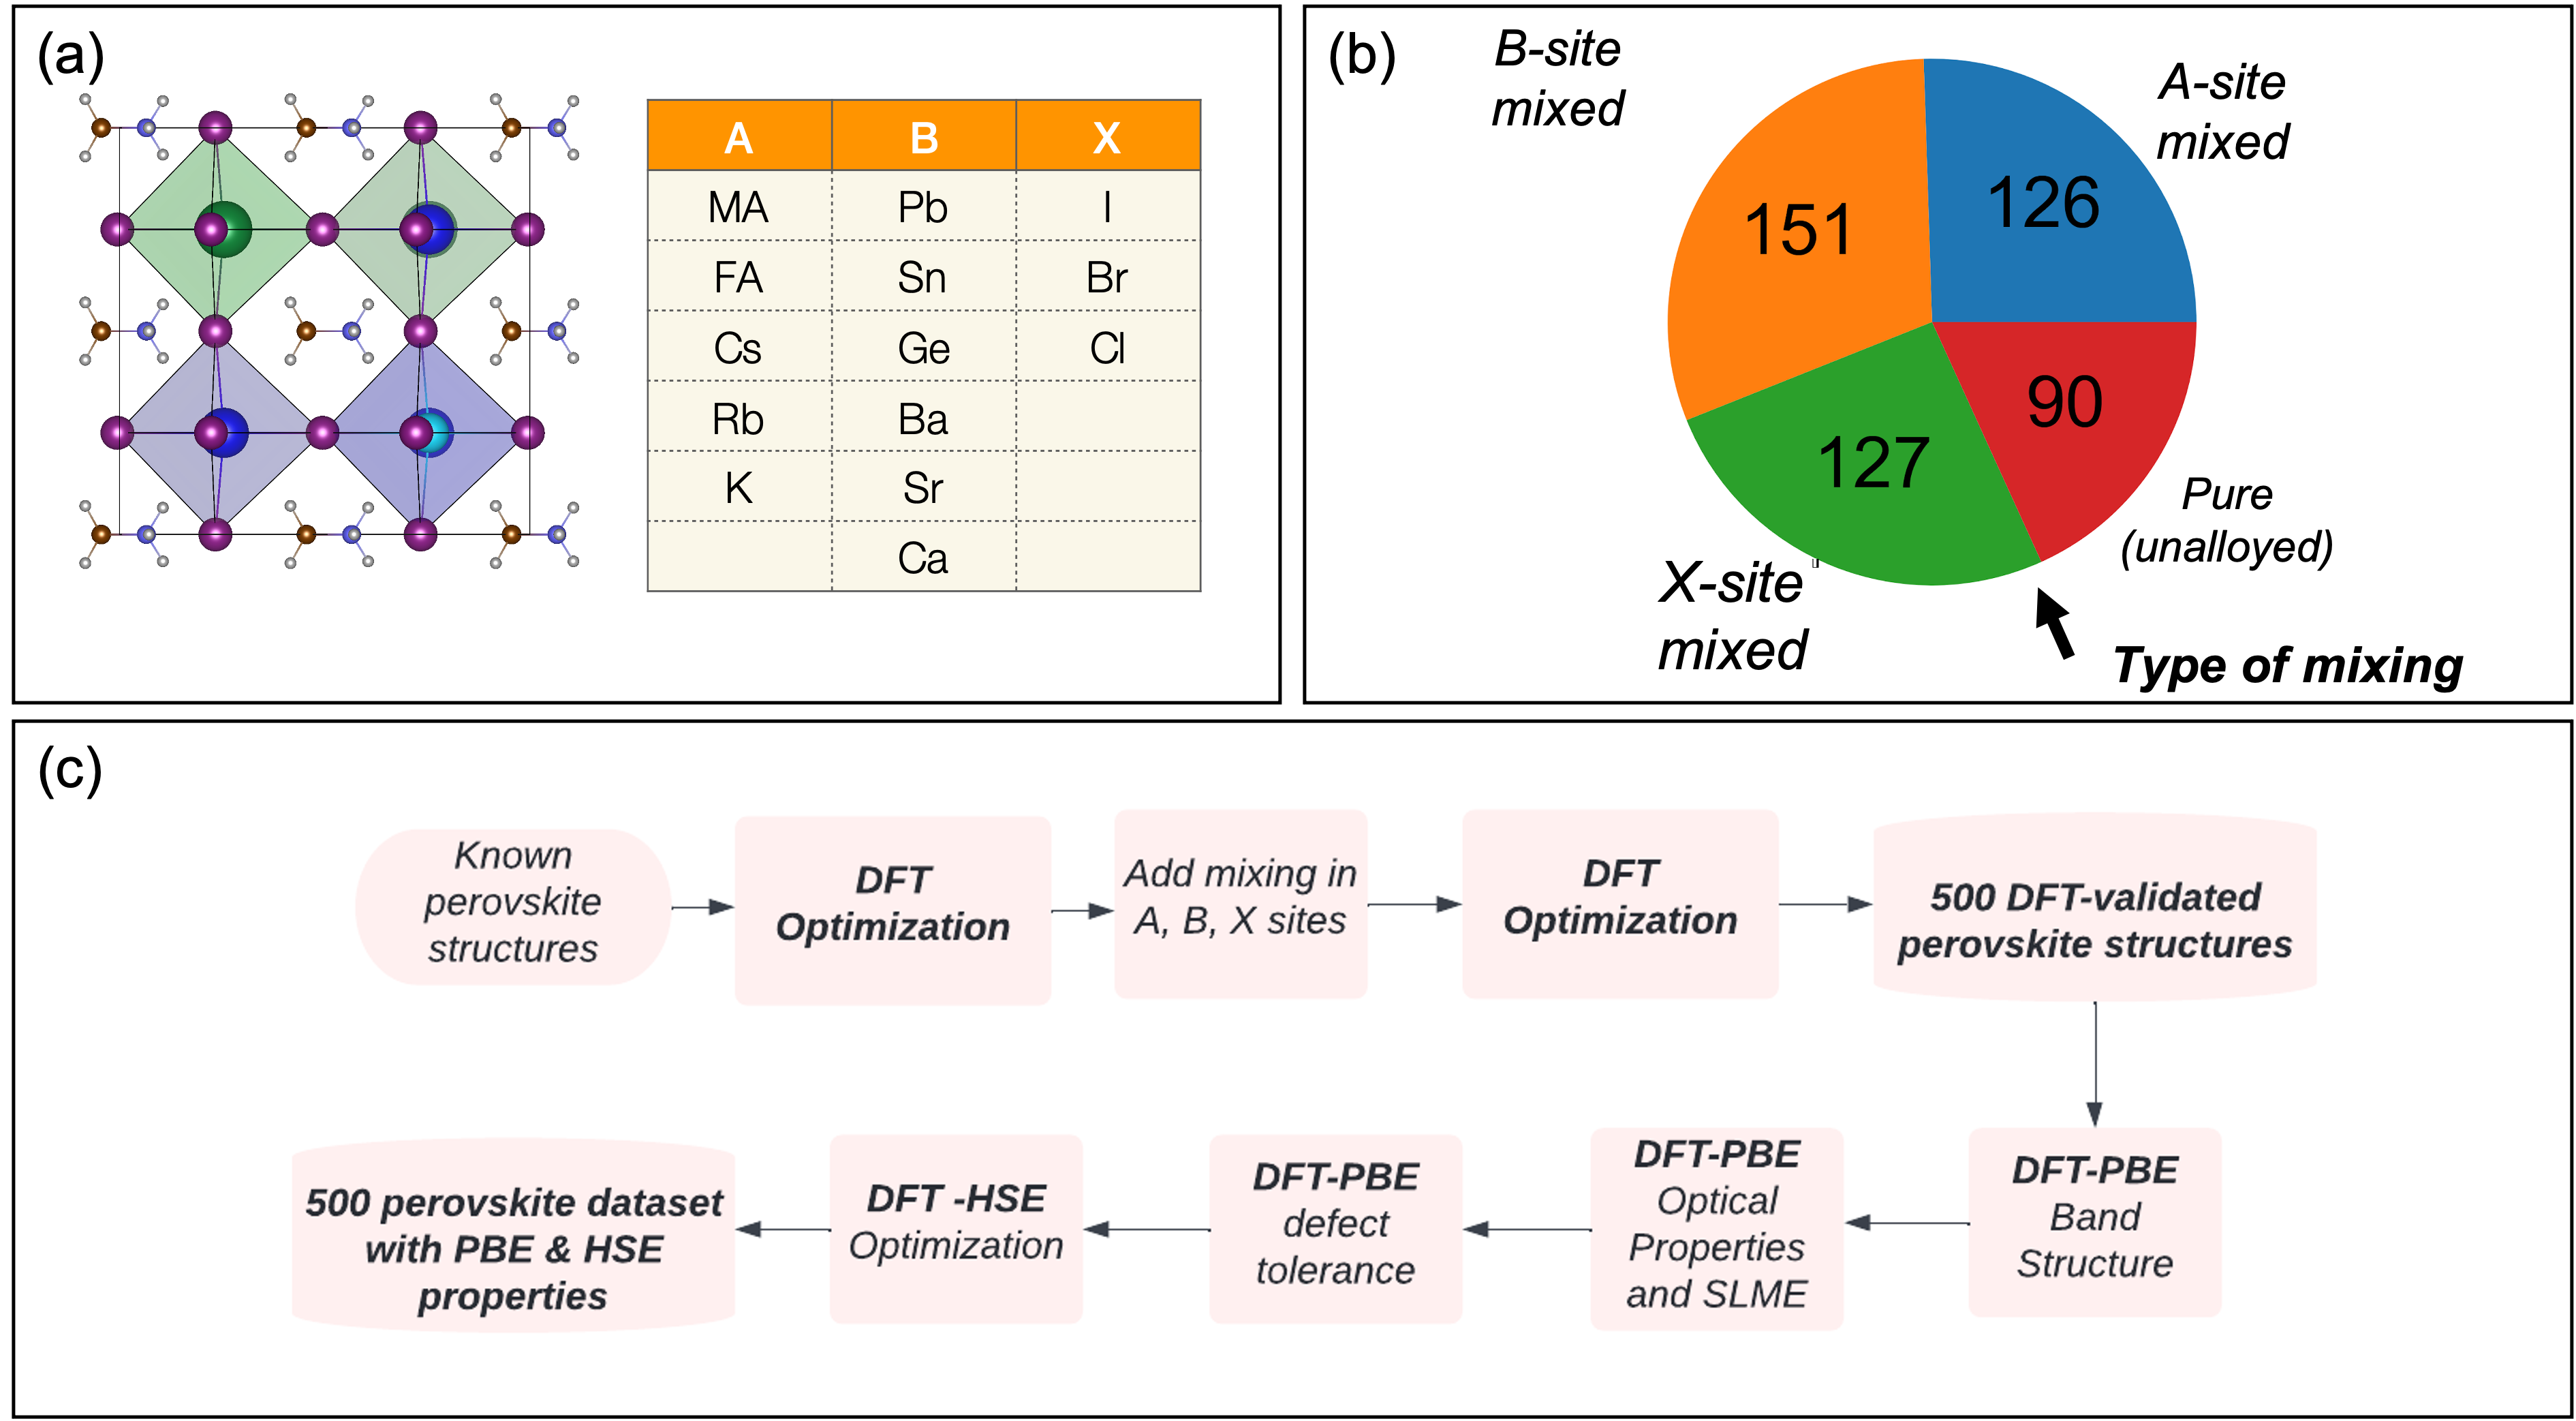
\includegraphics[width=0.99\linewidth]{Figure1.png}
\caption{\label{Fig:outline} 
(a) Chemical space of ABX$_3$ perovskites. (b) Pie charts showing the amounts of various atomic and molecular species as well as types of mixing in the DFT dataset. (c) Detailed outline of this work.}
\end{figure*}


\begin{figure*}[h]
\centering
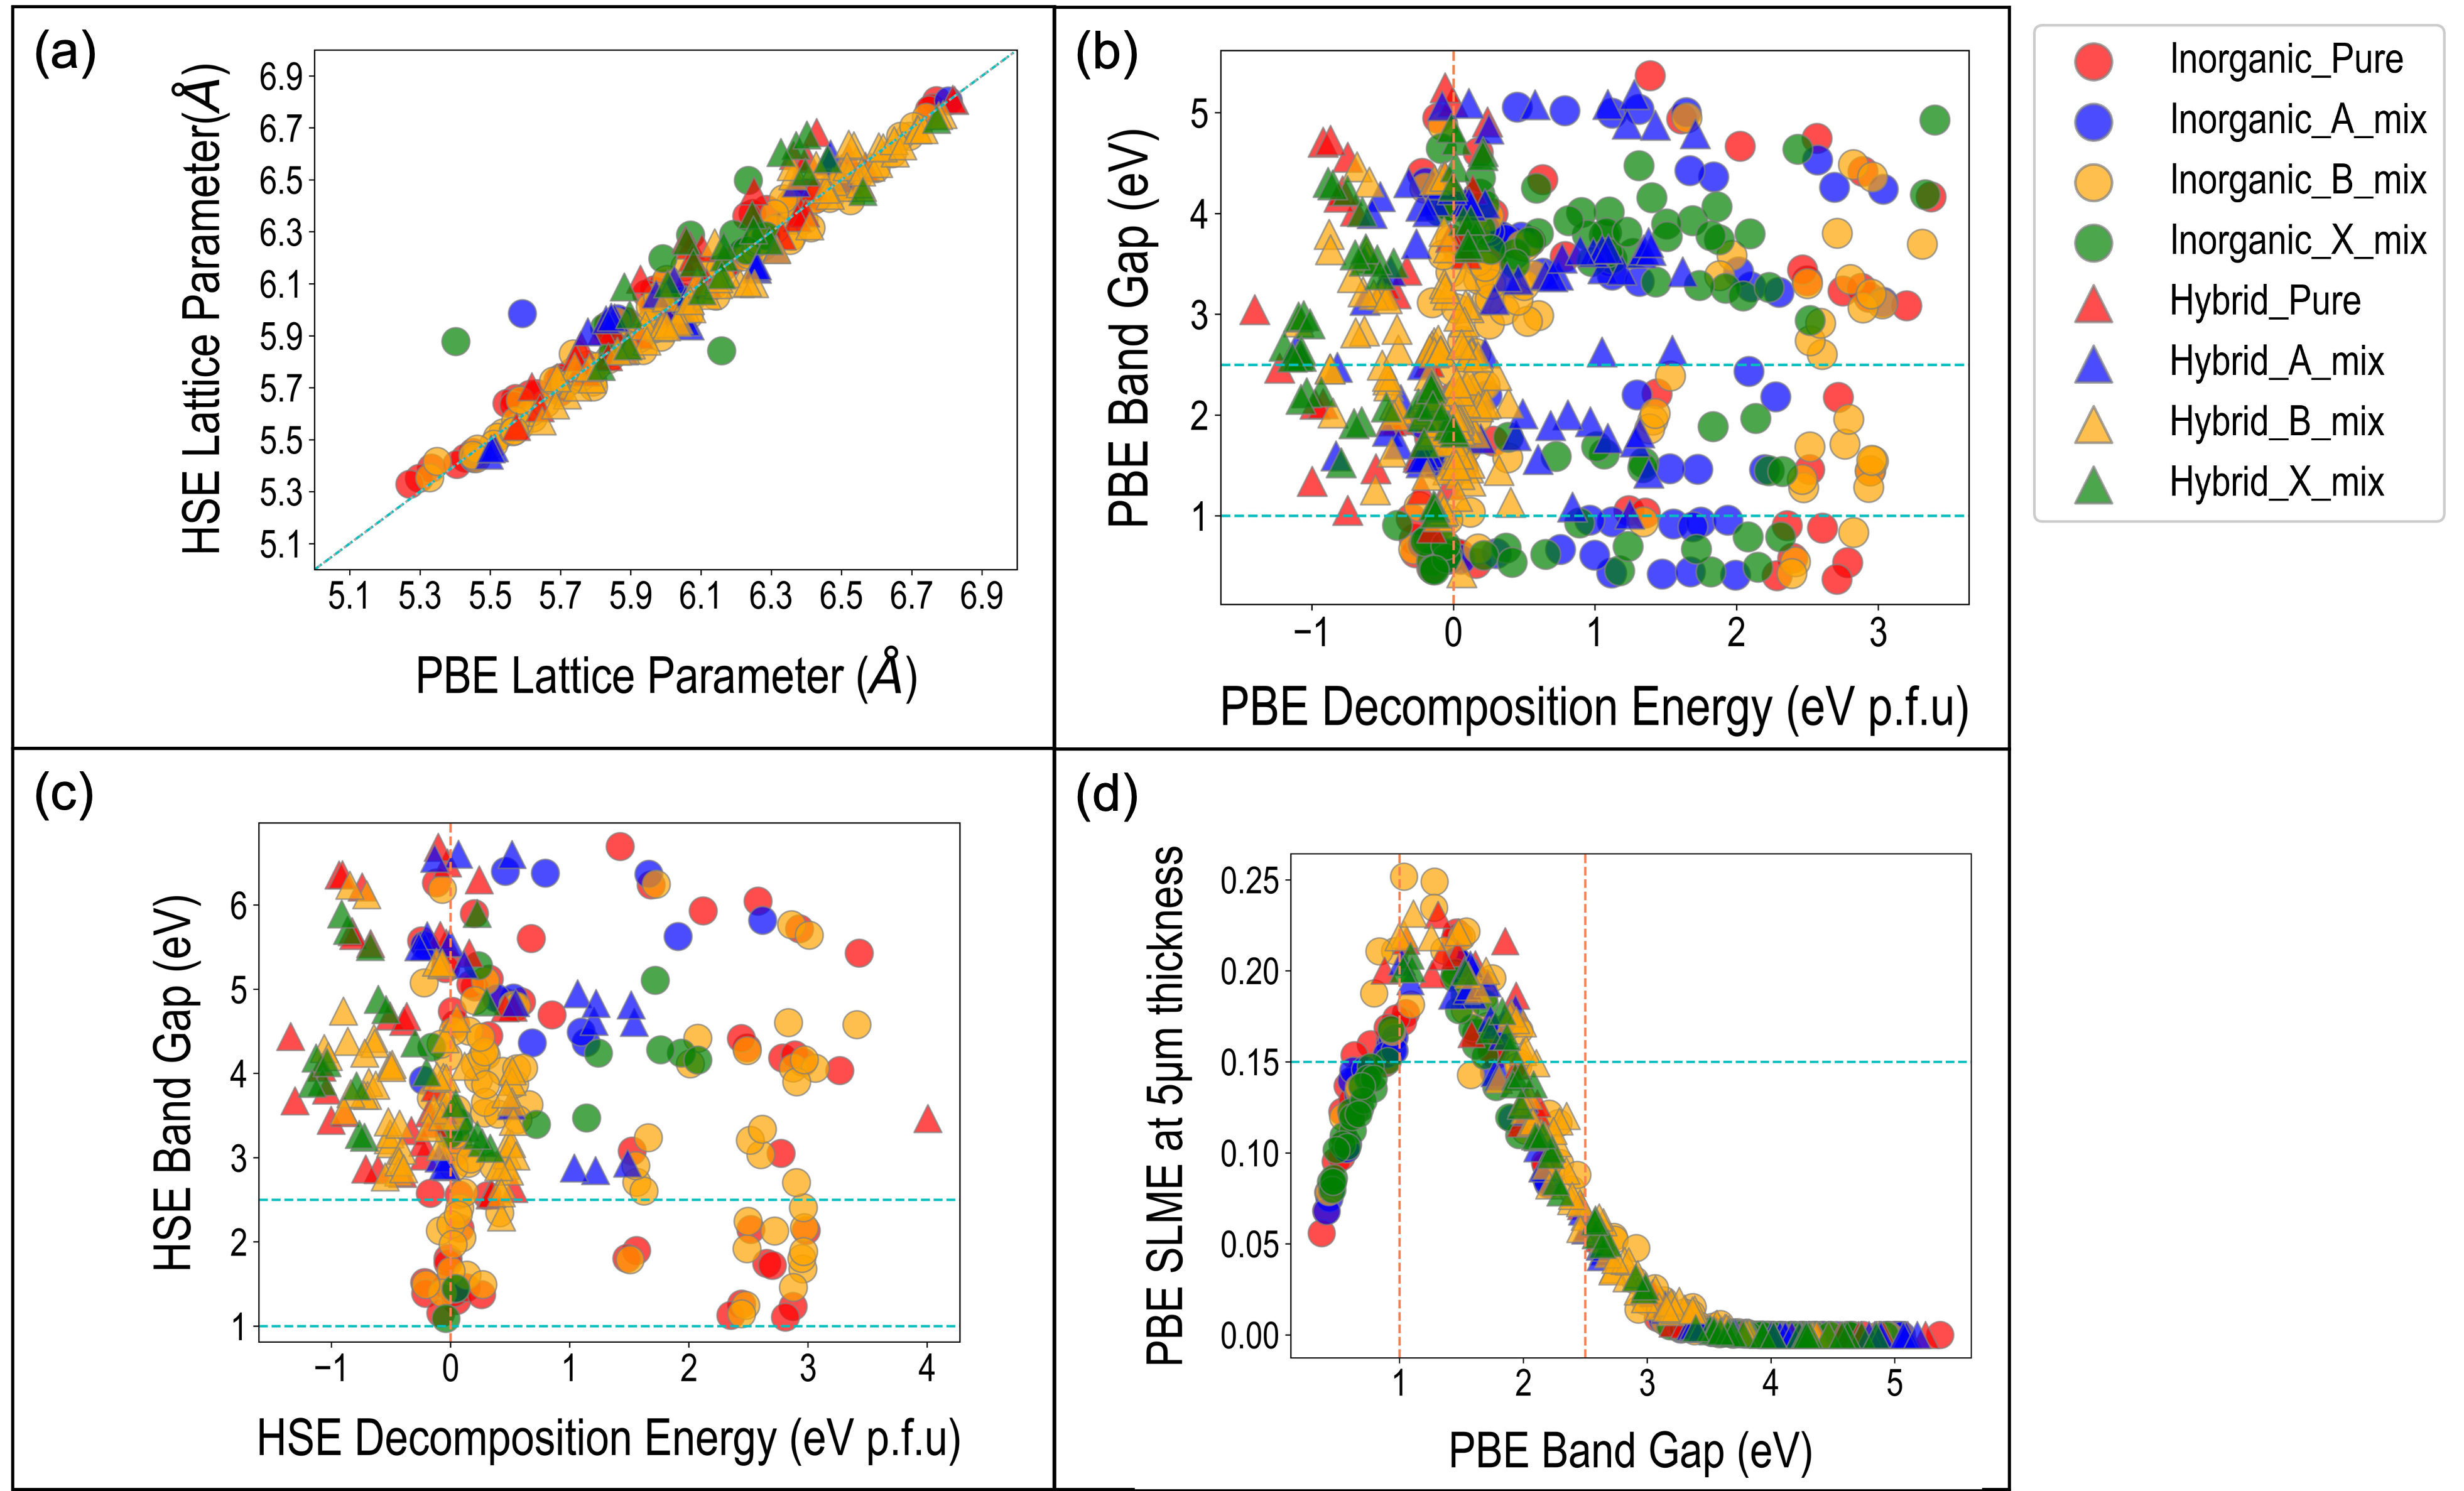
\includegraphics[width=0.99\linewidth]{Figure2.png}
\caption{\label{Fig:outline} 
Visualization of DFT data: PBE and HSE properties; lattice constants, decomposition energies, band gaps, photovoltaic figure of merit.}
\end{figure*}


\begin{figure*}[h]
\centering
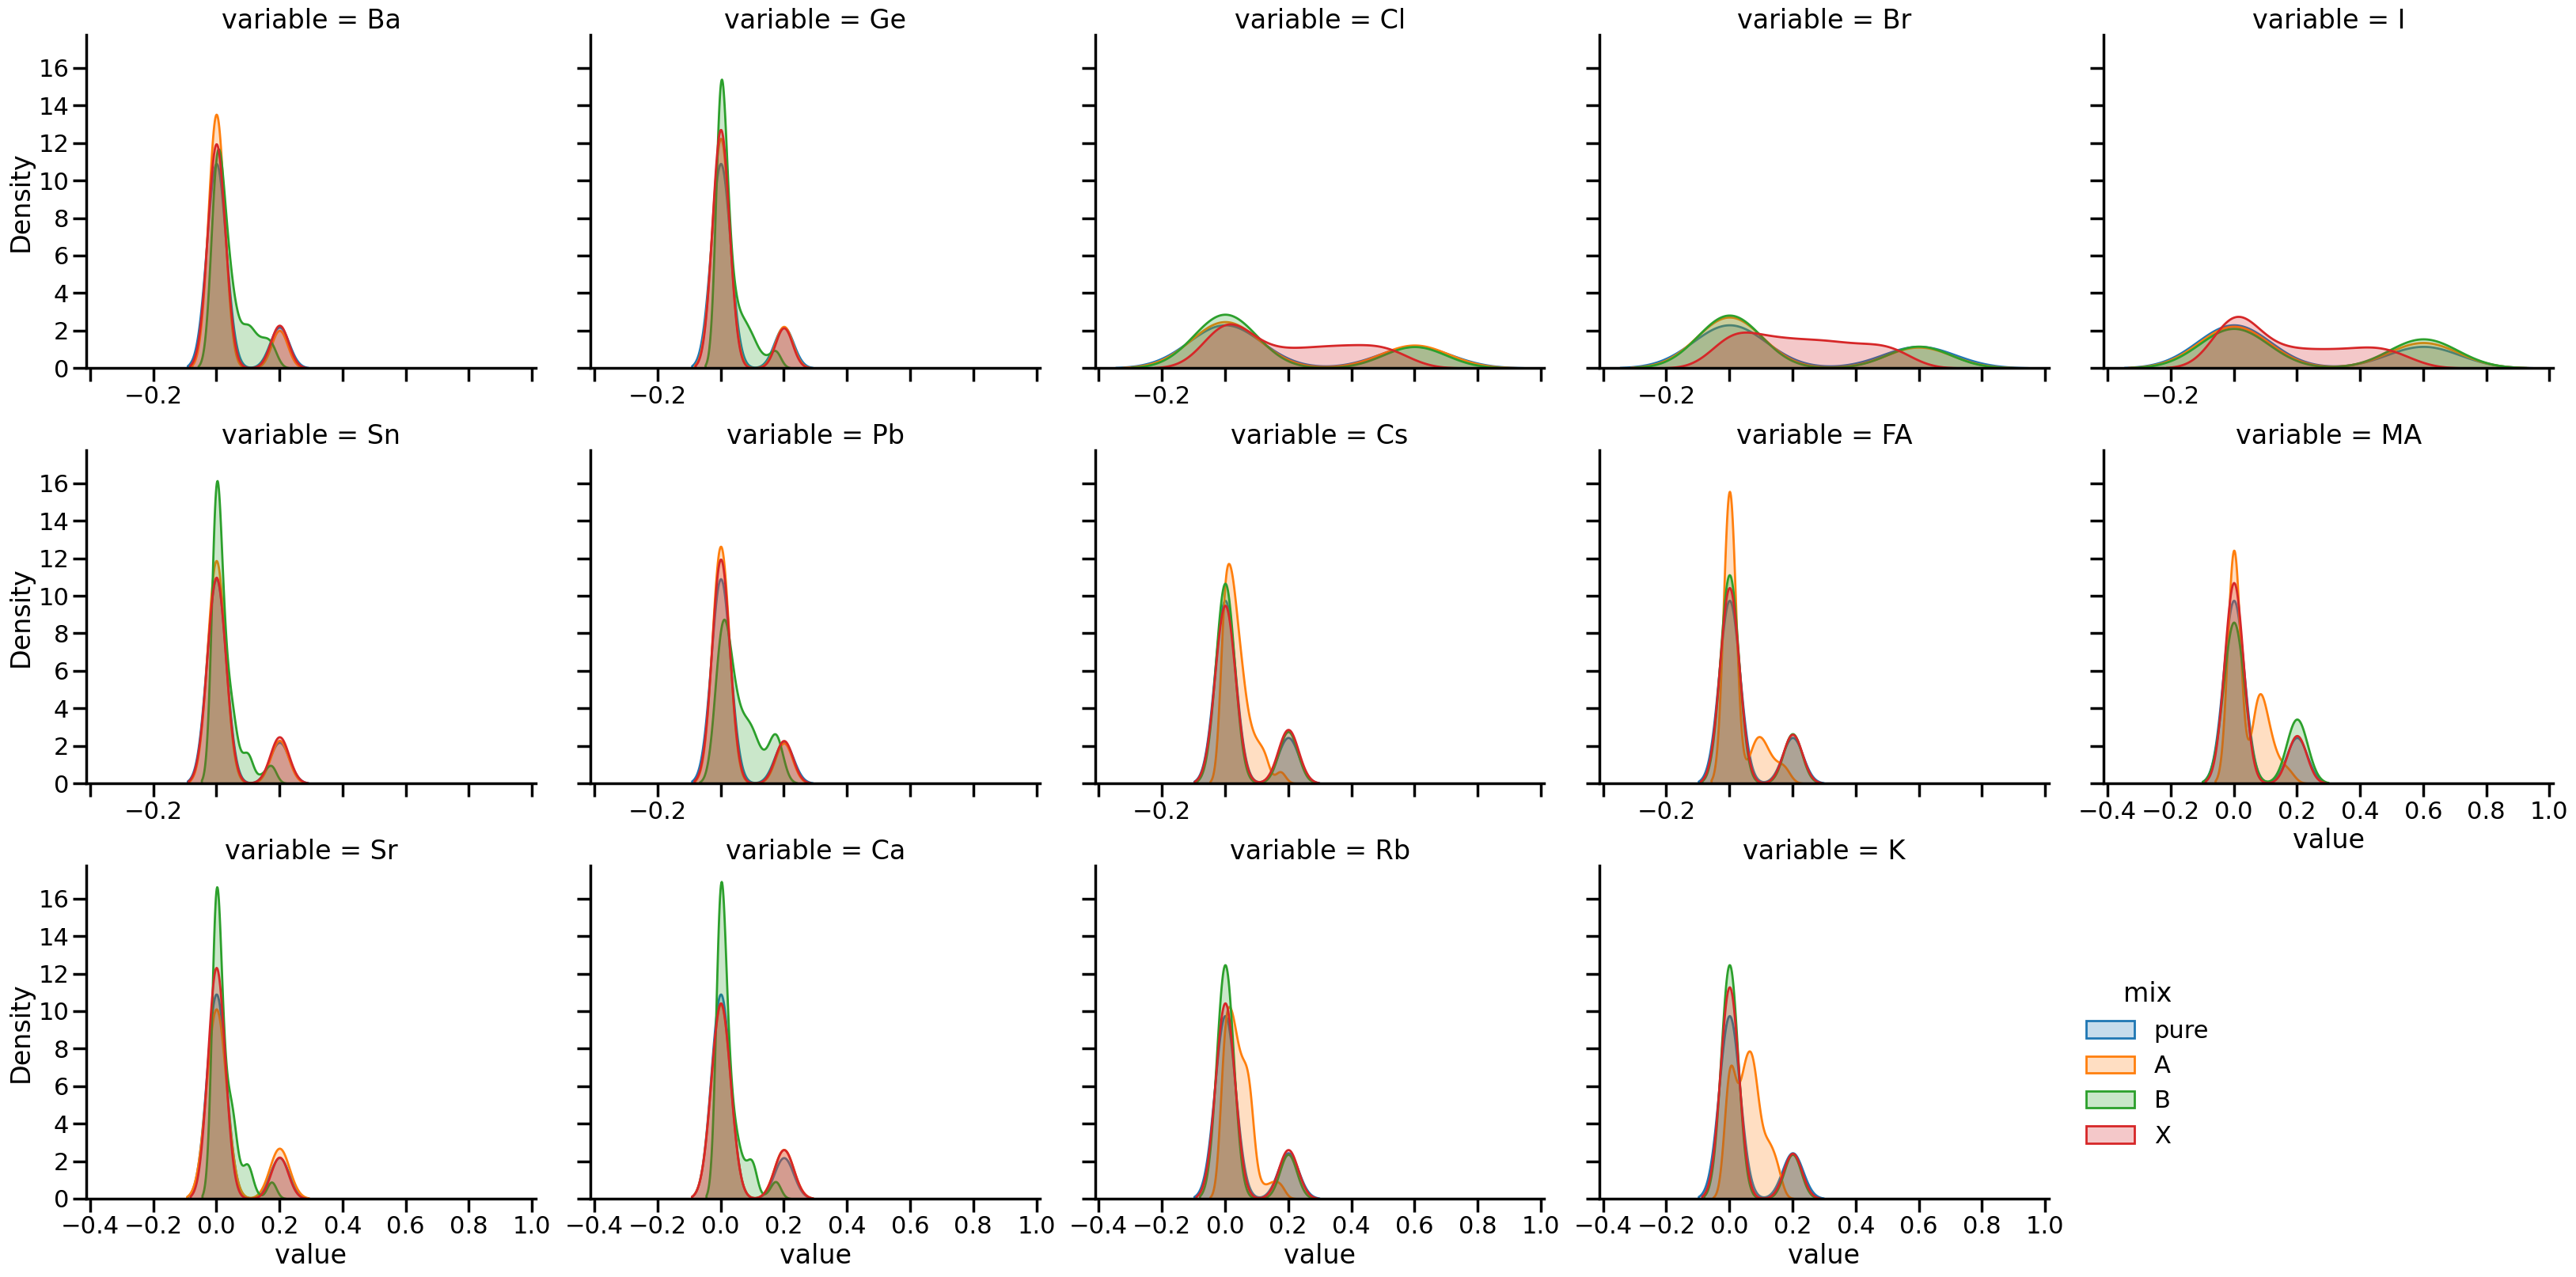
\includegraphics[width=0.80\linewidth]{./composition_kde.png}
\caption{\label{fig:kdes}
  Kernel Density Estimations with respect to main alloy classes of
  Perovskite Compositions }
\end{figure*}


\begin{figure*}[h]
\centering
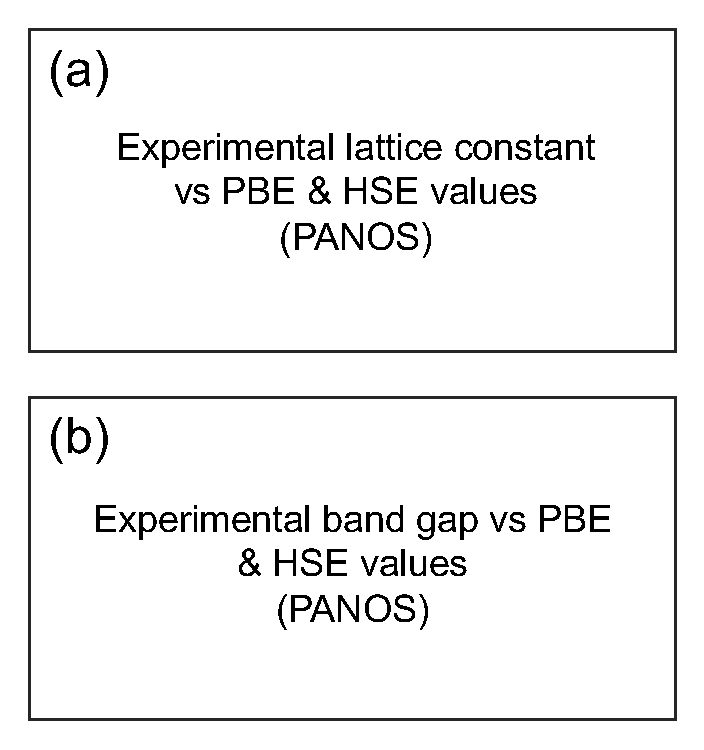
\includegraphics[width=0.80\linewidth]{Figure3.pdf}
\caption{\label{Fig:outline} 
Comparison of PBE and HSE computed properties with collected experimental measurements: (a) pseudo-cubic lattice constants, and (b) electronic band gaps.}
\end{figure*}


\begin{figure*}[h]
\centering
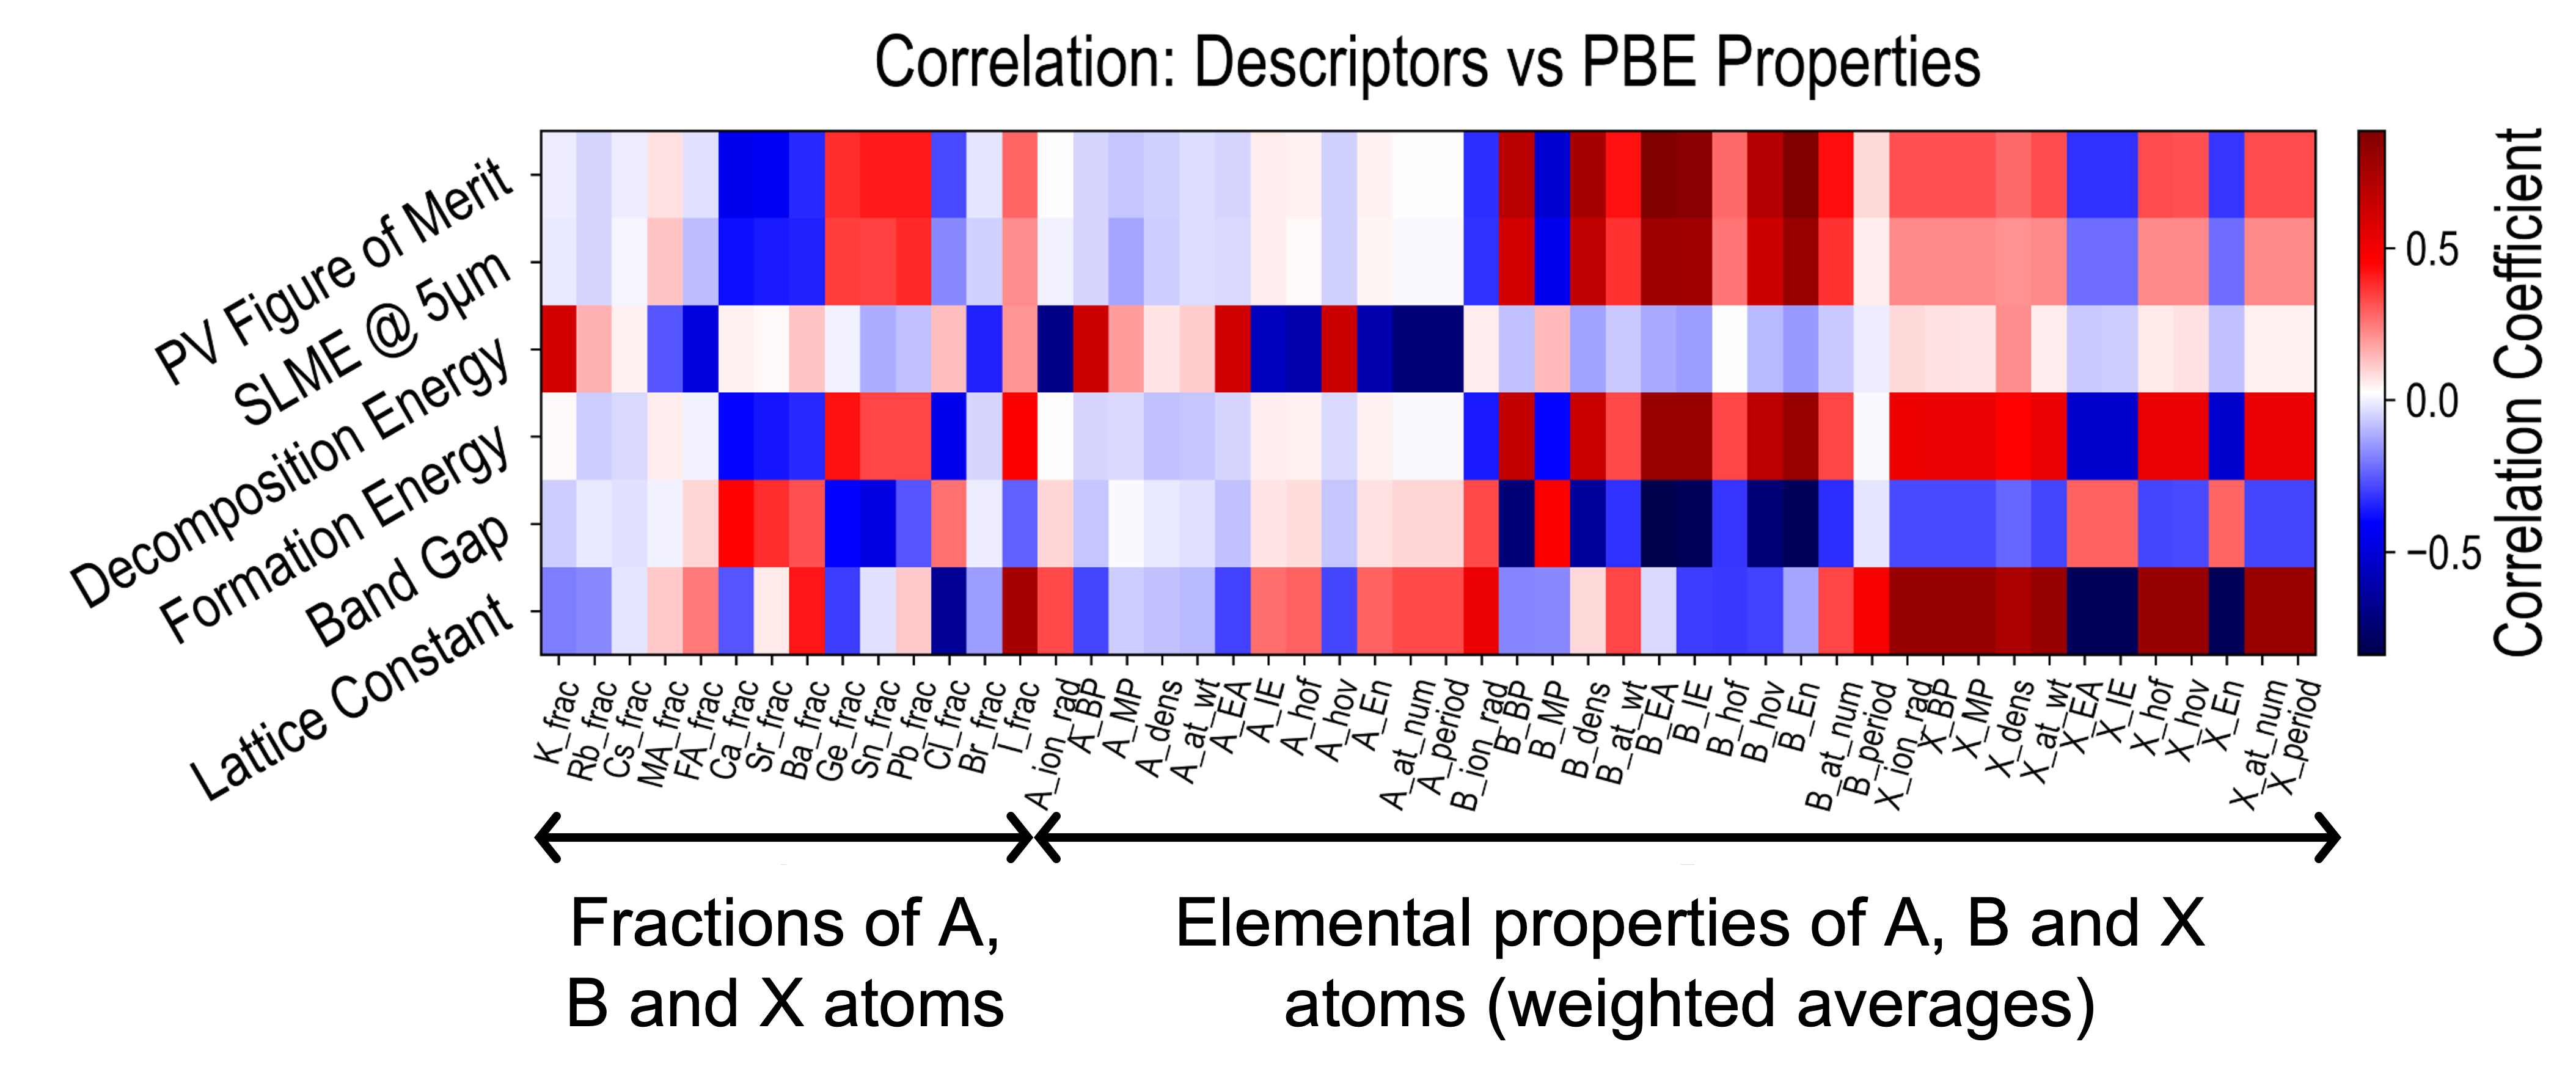
\includegraphics[width=0.99\linewidth]{Figure4.png}
\caption{\label{Fig:outline} 
Pearson linear correlation coefficients between 50 composition and elemental descriptors and (a) 6 PBE computed properties, and (b) 4 HSE computed properties.}
\end{figure*}


\begin{figure*}[h]
\centering
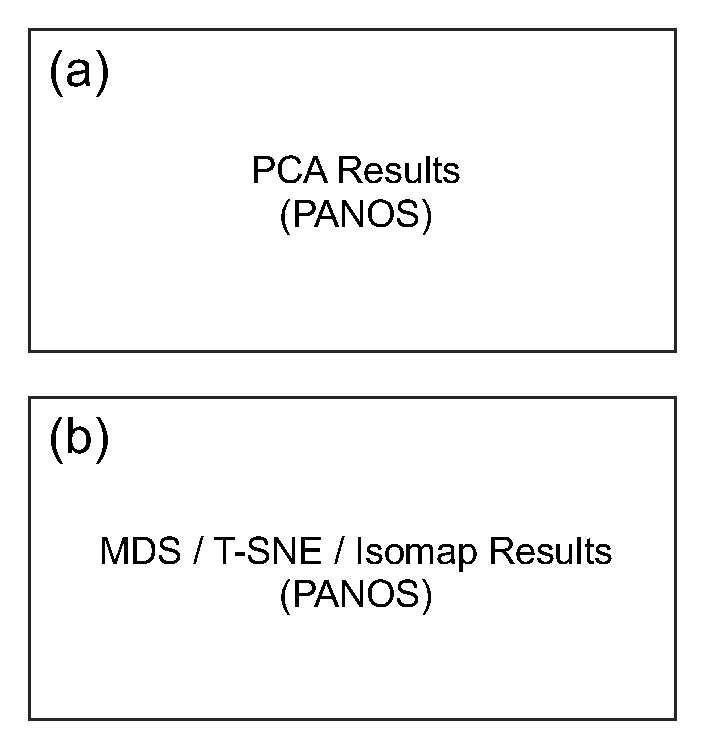
\includegraphics[width=0.80\linewidth]{Figure5.pdf}
\caption{\label{Fig:outline} 
Data visualization / dimensionality reduction / importance of features / trends in data using PCE, MDS, T-SNE, Isomap, etc.}
\end{figure*}


\begin{figure*}[h]
\centering
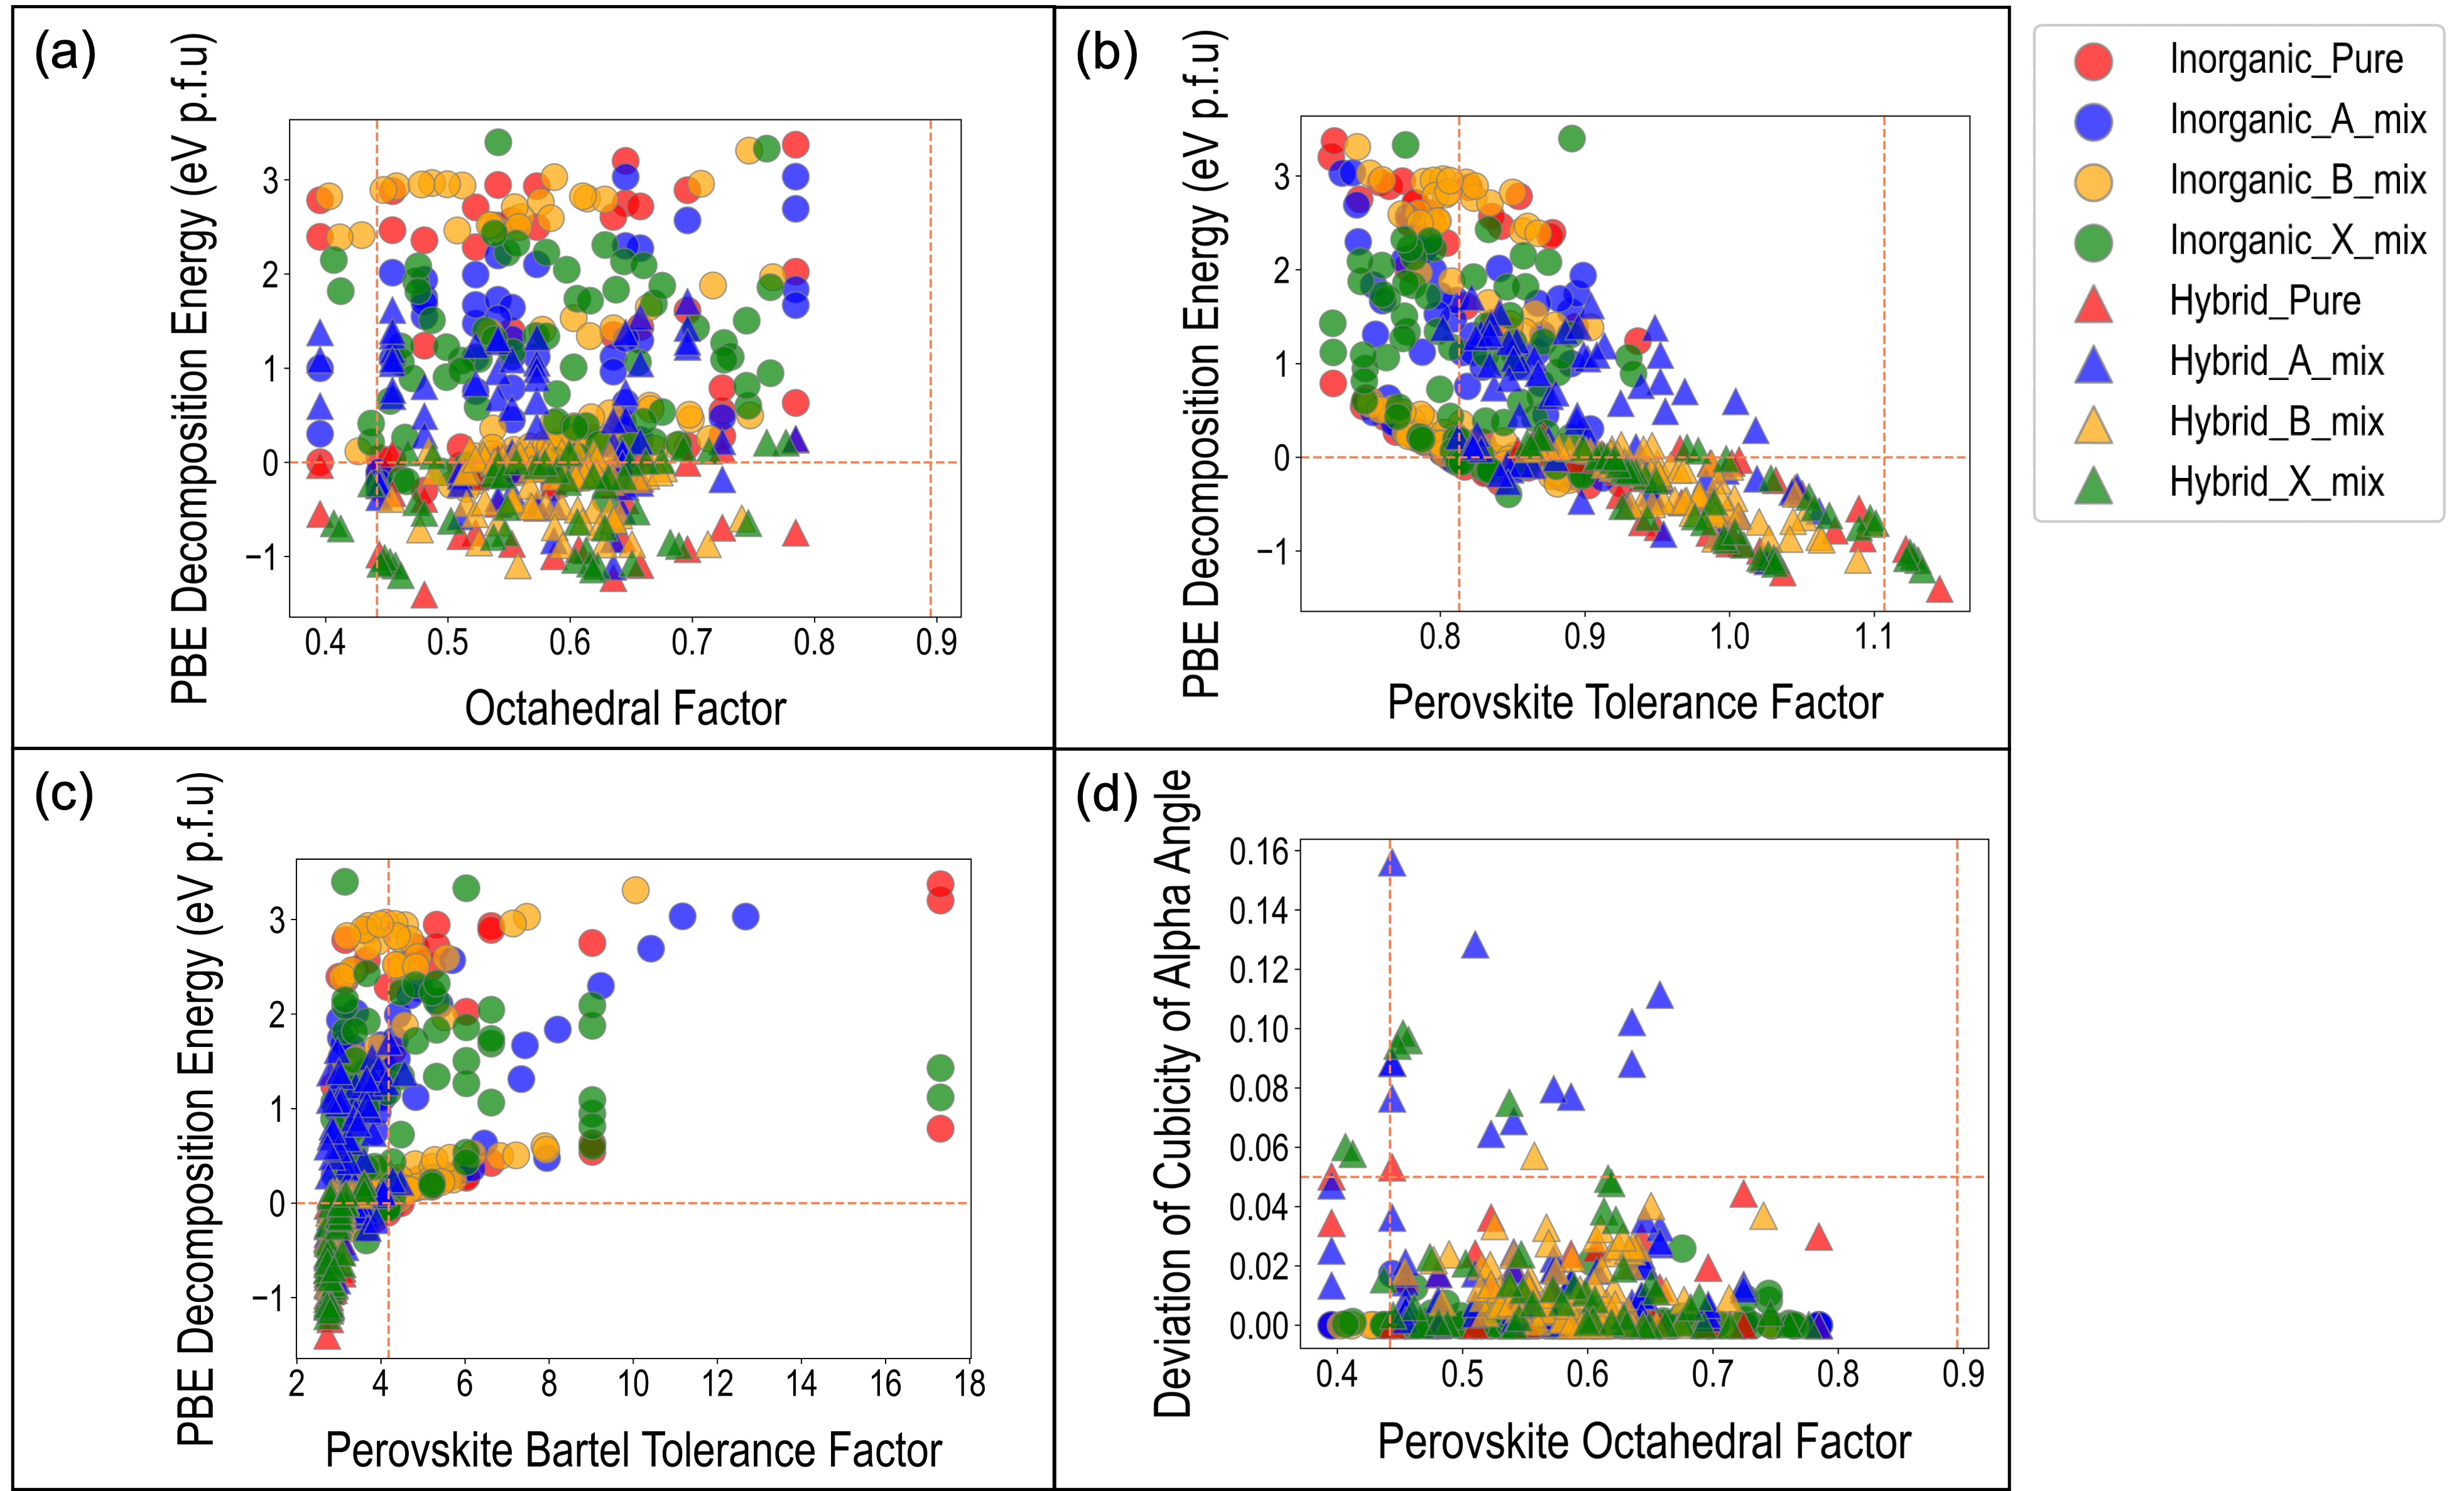
\includegraphics[width=0.99\linewidth]{Figure6.png}
\caption{\label{Fig:outline} 
Computed band structure, density of states, and optical absorption spectrum of 6 selected promising mixed composition perovskites.}
\end{figure*}


\newpage



\section*{Methodology}
% \begin{equation}\label{eqn-0}
% \begin{multlined}
% FOM = \sum_{\lambda_i} \alpha(\lambda_i) * I_s(\lambda_i) * (\lambda_{i+1} - \lambda_i) / \sum_{\lambda_i} I_s(\lambda_i) * (\lambda_{i+1} - \lambda_i)
% \end{multlined}
% \end{equation}
\subsection*{Building Perovskite Dataset}
Firstly, we start with known pure perovskite structures from public data base. 90 pure perovskites are constructed and DFT optimization are applied to get relaxed structures. Based on the pure perovskite structures, we add mixing for A, B, and X sites. To create mixing, for example in B sites, we first select possible B sites mixing elements. Then SQS methods are applied to generate random doping sties for given mixing concentrations. Thus, we constructed 126 A-site mixing samples, 151 B-site mixing samples and 127 X-site mixing samples. All samples are optimized by DFT calculations.

\subsection*{DFT Calculation Details}
DFT calculations are performed with Vienna Ab initio Simulation Package (VASP) version 5.4. The projector augmented wave (PAW) potentials were used The generalized gradient approximation (GGA) of Perdew, Burke and Ernzerhof (PBE) is used as exchange-correlation energy. The energy cutoff for the plane-wave basis is set to 500 eV. The Brillouin zone was sampled by Monkhorst-Pack k-point mesh, with a reciprocal mesh as 3x3x3. The structural force convergence threhold is set to be 0.025 eV/Å.

\subsection*{Properties Analysis}
\subsubsection*{Decomposition Energy}
The decomposition energy is an important property showing the stability of perovskite. To calculate the decomposition energy for ABX3 perovskite, we assume it will decompose to two phases, AX and BX2. Using DFT calculations, we can get the optimized energy of perovskite and its decomposed compounds.
%equation for decomposition energy
The equation is presenting the details calculation for decomposition energy. For PBE decomposition energy, we use DFT energy results from PBE level calculation. For HSE decomposition energy, we use the energy from HSE level calculations.
\subsubsection{Band Gap and Band Structure}

\subsubsection{LOPTICS Calculations and Absorption Spectrum}

\subsubsection{SLME Package}

\subsubsection{Dielectric Constant }

\newpage




\section*{Results and discussion}

\subsection*{Visualization of DFT Data / Explanation of Trends}

\subsection*{Pearson Correlation Results}

\subsection*{PCA / MDS / T-SNE / Isomap Results}

\subsection*{Band Structure and Absorption Spectrum of Selected Compounds}

... \\

% \begin{table}
% \centering
%   \caption{\ NN model training and test prediction RMSEs for every property.}
%   \label{table:rmse}
%   \begin{tabular}{ccc}
%     \hline
%   &   &   \\
% \textbf{Property}  &  \textbf{Training Set RMSE}  &  \textbf{Test Set RMSE} \\
%   &   &   \\
% \hline
%   &   &   \\
%       PBE Lattice Constant  & 0.09 \AA  & 0.10 \AA  \\
%       HSE Lattice Constant  & 0.06 \AA  & 0.06 \AA  \\
%       $\Delta$H$_{decomp}$ (PBE) & 0.05 eV  & 0.11 eV  \\
%       $\Delta$H$_{decomp}$ (HSE)  & 0.05 eV  & 0.09 eV  \\
%       E$_{gap}$$^{PBE}$  & 0.20 eV  & 0.22 eV  \\
%       E$_{gap}$$^{HSE}$  & 0.19 eV  & 0.24 eV  \\
%       Refractive Index  & 0.04  & 0.05  \\
%       PV FOM (log$_{10}$)  & 0.14  & 0.18  \\
%       X-rich D.F.E.  & 0.12 eV  & 0.23 eV  \\
%       X-rich E$_{F}$  & 0.06 eV  & 0.19 eV  \\
%       Medium-X D.F.E.  & 0.18 eV  & 0.29 eV  \\
%       Medium-X E$_{F}$  & 0.11 eV  & 0.30 eV  \\
%       B-rich D.F.E.  & 0.11 eV  & 0.30 eV  \\
%       B-rich E$_{F}$  & 0.11 eV  & 0.25 eV  \\
%       V$_{A}$ (0/-1) & 0.07 eV  & 0.11 eV  \\
%       V$_{X}$ (+1/0)  & 0.19 eV  & 0.22 eV  \\
%   &   &   \\
%     \hline
%   \end{tabular}
% \end{table}

\newpage



\section*{Perspective and Future Work}
    
... \\



\section*{Conclusions}

... \\


\section*{Conflicts of interest}
There are no conflicts to declare.

\section*{Acknowledgements}
Extensive discussions with and scientific feedback from UC San Diego researchers David Fenning and Rishi Kumar and Argonne National Lab scientist Maria Chan are acknowledged. This work was performed at Purdue University, under startup account F.10023800.05.002 from the Materials Engineering department. This research used resources of the National Energy Research Scientific Computing Center, the Laboratory Computing Resource Center at Argonne National Laboratory, and the RCAC clusters at Purdue.


\balance


\bibliography{rsc} %You need to replace "rsc" on this line with the name of your .bib file
\bibliographystyle{rsc} %the RSC's .bst file





\clearpage
\newpage
\setcounter{page}{1}

%\onecolumngrid

\setcounter{figure}{0}   
\setcounter{table}{0} 
\renewcommand{\thetable}{S\Roman{table}} 
\renewcommand\thefigure{S\arabic{figure}}
 
\begin{center}
\vspace*{0.5cm}
\Large
\textbf{Supplemental material to "A High-Throughput Computational Dataset of Halide Perovskite Alloys"\\}
\vspace{0.5cm}
\large
Jiaqi Yang,\textit{$^{a}$} Panayotis Manganaris\textit{$^{a}$} and Arun Mannodi-Kanakkithodi\textit{$^{a}$} \\
\vspace{0.3cm}

\normalsize
\textsuperscript{a}\textit{School of Materials Engineering, Purdue University, West Lafayette, Indiana 47907, USA} \\
\end{center}

\footnote{
\textsuperscript{a}amannodi@purdue.edu\hspace{0.3cm}}

\vspace{1cm}



% \begin{figure*}[h]
% \centering
% \includegraphics[width=\linewidth]{SI_figs/Table_elem_prop.pdf}
% \caption{\label{Fig:SI_elem_prop} 
% List of 15 elemental/molecular properties and tabulated values used for each A, B and X-site constituent in the halide perovskite chemical space.}
% \end{figure*}


% \begin{table*}[h]
% \centering
%   \caption{\ Calculated PV figures of merit (in log$_{10}$) for known semiconductors and some selected compounds from the current study.}
%   \label{table:SI_FOM}
%   \begin{tabular}{cc}
%     \hline
%   &   \\
% \textbf{Compound}  &  \textbf{log$_{10}$ (PV FOM)} \\
%   &   \\
% \hline
%   &   \\
% Si    &   5.64   \\
% SiC   &   3.76   \\
% GaAs   &   5.66   \\
% CdTe   &   5.46   \\
% CdSe   &   5.31   \\
% 	   &   \\
% CsCa$_{0.25}$Ba$_{0.125}$Ge$_{0.25}$Pb$_{0.375}$Cl$_{3}$   &   4.72   \\
% MACa$_{0.375}$Ge$_{0.5}$Pb$_{0.125}$Br$_{3}$   &   4.88   \\
% MACa$_{0.125}$Sr$_{0.125}$Ba$_{0.125}$Ge$_{0.125}$Pb$_{0.5}$I$_{3}$   &   5.07   \\
% CsCa$_{0.875}$Pb$_{0.125}$Br$_{3}$   &   3.84   \\
% FACa$_{0.125}$Sr$_{0.375}$Ba$_{0.125}$Sn$_{0.125}$Pb$_{0.25}$I$_{3}$   &   4.88   \\
%   &   \\
%     \hline
%   \end{tabular}
% \end{table*}

\end{document}
